\documentclass[pagenumbers=false]{goose-article}

\setcounter{topnumber}{2}
\setcounter{bottomnumber}{2}
\setcounter{totalnumber}{4}
\renewcommand{\topfraction}{0.85}
\renewcommand{\bottomfraction}{0.85}
\renewcommand{\textfraction}{0.15}
\renewcommand{\floatpagefraction}{0.8}
\renewcommand{\textfraction}{0.1}
\setlength{\floatsep}{5pt plus 2pt minus 2pt}
\setlength{\textfloatsep}{5pt plus 2pt minus 2pt}
\setlength{\intextsep}{5pt plus 2pt minus 2pt}

\title{Creep at a frictional interface}
\author{Tom de Geus}
\hypersetup{pdfauthor={T.W.J. de Geus}}

\begin{document}

\twocolumn[
    \begin{@twocolumnfalse}
        \maketitle
    \end{@twocolumnfalse}
]
\sloppy

\paragraph{Impact}

Understanding how slip at a frictional interface initiates is important for e.g.~earthquake prediction and precision engineering.
It is commonly accepted that the ``static friction coefficient'' grows in time due to creep.
However, it remains a mystery how creep relates the spontaneous slip nucleation.

\paragraph{Measurements}

Spontaneous slip nucleation happens when the system is driven using a weak spring.
The system then displays stick-slip.
However, although creep is present, its effect is not trivially observed as stick-slip is quasi-periodic.
We propose a setup in which multiple, coupled, interfaces are driven by weak springs, see below.
This forces the stick-slip cycles to de-synchronize, such that the effect of creep becomes visible and the creep rate can be measured.

\begin{figure}[htp]
    \centering
    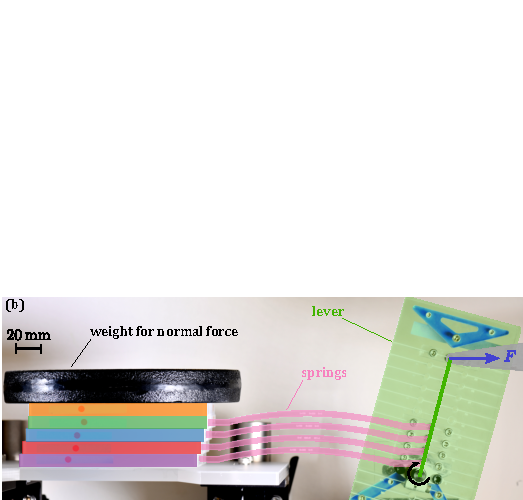
\includegraphics[width=\linewidth]{setup.pdf}
\end{figure}

\paragraph{Model}

The simplest model is that of an elastic interface driven over a disordered pinning potential.
It consists of $N$ particles that interact interact with their nearest neighbours.
Each particle, furthermore, experiences a driving force (by connecting the particle to a driving frame using a weak spring) and an elastic force due to the pinning potential.

\paragraph{Depinning}

In the overdamped limit, such a model displays a depinning transition.
The system is pinned below a critical driving force, and slips above it.
At the critical force, the system displays critical behaviour, i.e.~the correlation length diverges.
Thereby, the dynamics are intermittent: it displays avalanches whose size, extent, and duration, are power-law distributed.
Under these assumptions, the exponents are now well understood.
What happens in the presence of inertia and temperature is less clear.

\paragraph{Thermal avalanches}

Still neglecting inertia, but assuming a finite temperature, the system displays creep at any force: the depinning transition is ``rounded''.
Intriguingly, the creep regime is also intermittent.
Due to elastic coupling the activations are spatially correlated: thermal avalanches occur, see below (showing activity at different times at a fixed temperature, left, and at different temperatures at fixed time, right).
We predict these exponents to be the same exponents as the depinning transition itself.

\begin{figure}[htp]
    \centering
    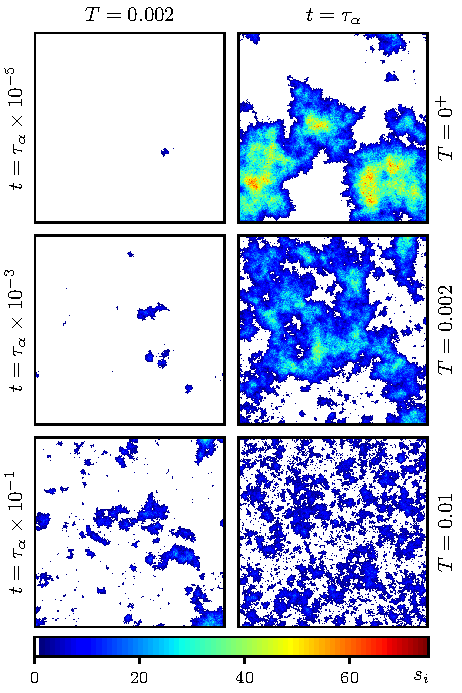
\includegraphics[width=0.9\linewidth]{prl_snapshots.pdf}
\end{figure}

\nocite{Poincloux2023,deGeus2024}
\bibliographystyle{unsrtnat}
\renewcommand{\refname}{Selection of publications}
\bibliography{library}

\end{document}
